\documentclass[10pt, aspectratio=169]{beamer}
\usepackage[utf8]{inputenc}
\usepackage[spanish]{babel}
\usepackage{graphicx}
\usepackage{hyperref}
\usepackage{fontawesome5}
\usepackage{xcolor}
\usepackage{caption}

% Tema limpio y profesional
\usetheme{Madrid}
\usecolortheme{default}
\setbeamertemplate{navigation symbols}{}
\setbeamertemplate{footline}[frame number]

% Colores personalizados
\definecolor{main}{HTML}{6B4EFF}
\definecolor{accent}{HTML}{FF6B6B}

\setbeamercolor{structure}{fg=main}
\setbeamercolor{title}{fg=main}

\title{\textbf{Smart Notes}}
\subtitle{Aplicación de Notas Inteligente con IA}
\author{Aaron Rodrigo Ramos Reyes}
\institute{Universidad Autónoma Metropolitana \\ Unidad Cuajimalpa \\ Interacción Humano-Computadora}
\date{\today}

\begin{document}

% Diapositiva de Título
\begin{frame}
    \titlepage
\end{frame}

% Índice
\begin{frame}{Contenido}
    \tableofcontents
\end{frame}

% 1. Introducción
\section{Introducción}
\begin{frame}{¿Qué es Smart Notes?}
    \begin{itemize}
        \item Aplicación móvil para crear y organizar notas personales
        \item Enfocada en \textbf{productividad inteligente}
        \item Diseño \textbf{minimalista} y moderno
        \item Funcionalidades avanzadas de interacción táctil
    \end{itemize}
    
    \vspace{1em}
    \centering
    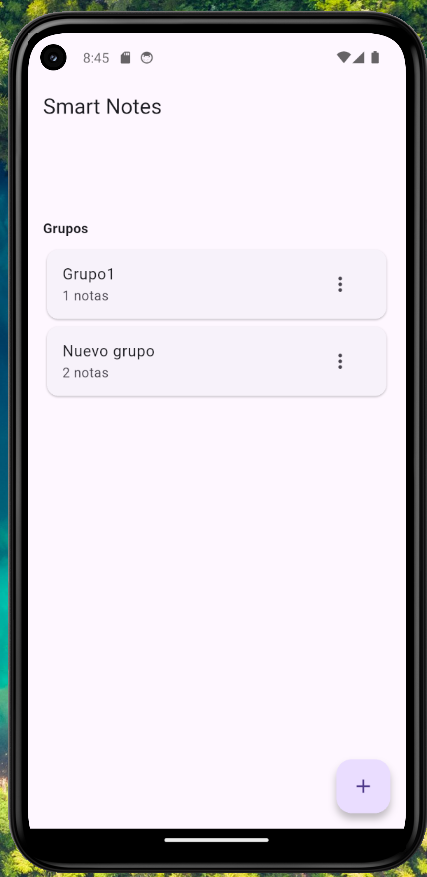
\includegraphics[width=0.65\textwidth]{imagenes/home.png}
\end{frame}

% 2. Tecnologías Utilizadas
\section{Tecnologías}
\begin{frame}{Tecnologías Utilizadas}
    \begin{columns}
        \column{0.5\textwidth}
        \begin{itemize}
            \item \faCode\ Flutter + Dart
            \item \faDatabase\ Hive (Base de datos local)
            \item \faBell\ Notificaciones locales
            \item \faRobot\ OpenRouter (Inteligencia Artificial)
        \end{itemize}
        \column{0.5\textwidth}
        \centering
        
\includegraphics[width=0.8\textwidth]{imagenes/flutter_logo.png} % opcional
    \end{columns}
\end{frame}

% 3. Arquitectura
\section{Arquitectura}
\begin{frame}{Arquitectura del Proyecto}
    \begin{itemize}
        \item \textbf{Capa de Presentación}: Pantallas y widgets
        \item \textbf{Capa de Negocio}: Servicios e IA (\texttt{AIService}, \texttt{IntelligentAssistant})
        \item \textbf{Capa de Datos}: Modelos + Hive
    \end{itemize}
    
    \vspace{0.8em}
    \centering
    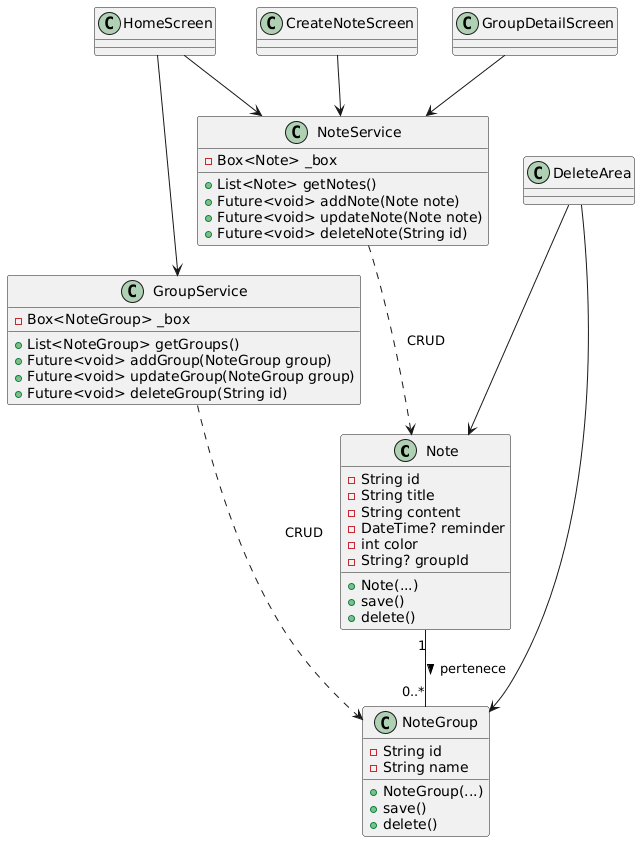
\includegraphics[width=0.85\textwidth]{imagenes/clases.png}
    \captionof{figure}{Diagrama de clases principal}
\end{frame}

% 4. Funcionalidades Principales
\section{Funcionalidades}
\begin{frame}{Funcionalidades Principales}
    \begin{itemize}
        \item Creación y edición de notas con colores personalizados
        \item Sistema de \textbf{grupos} (carpetas)
        \item Historial de edición (Undo / Redo)
        \item \textbf{Arrastrar y soltar} avanzado:
        \begin{itemize}
            \item Nota sobre nota → crear grupo automático
            \item Nota sobre grupo → asignar automáticamente
            \item Arrastrar a zona superior → eliminar con confirmación
        \end{itemize}
        \item Notificaciones locales
    \end{itemize}
\end{frame}

% 5. Integración con IA (OpenRouter)
\section{Inteligencia Artificial}
\begin{frame}{Integración con OpenRouter}
    \begin{itemize}
        \item Uso de la API de OpenRouter para análisis inteligente
        \item Al guardar una nota se envía título y contenido
        \item La IA responde en formato JSON estructurado
        \item Sugiere automáticamente:
        \begin{itemize}
            \item Configurar \textbf{alarmas} detectando fechas
            \item Crear o mover a \textbf{grupos} temáticos
        \end{itemize}
    \end{itemize}
    
    \vspace{1em}
    \centering
    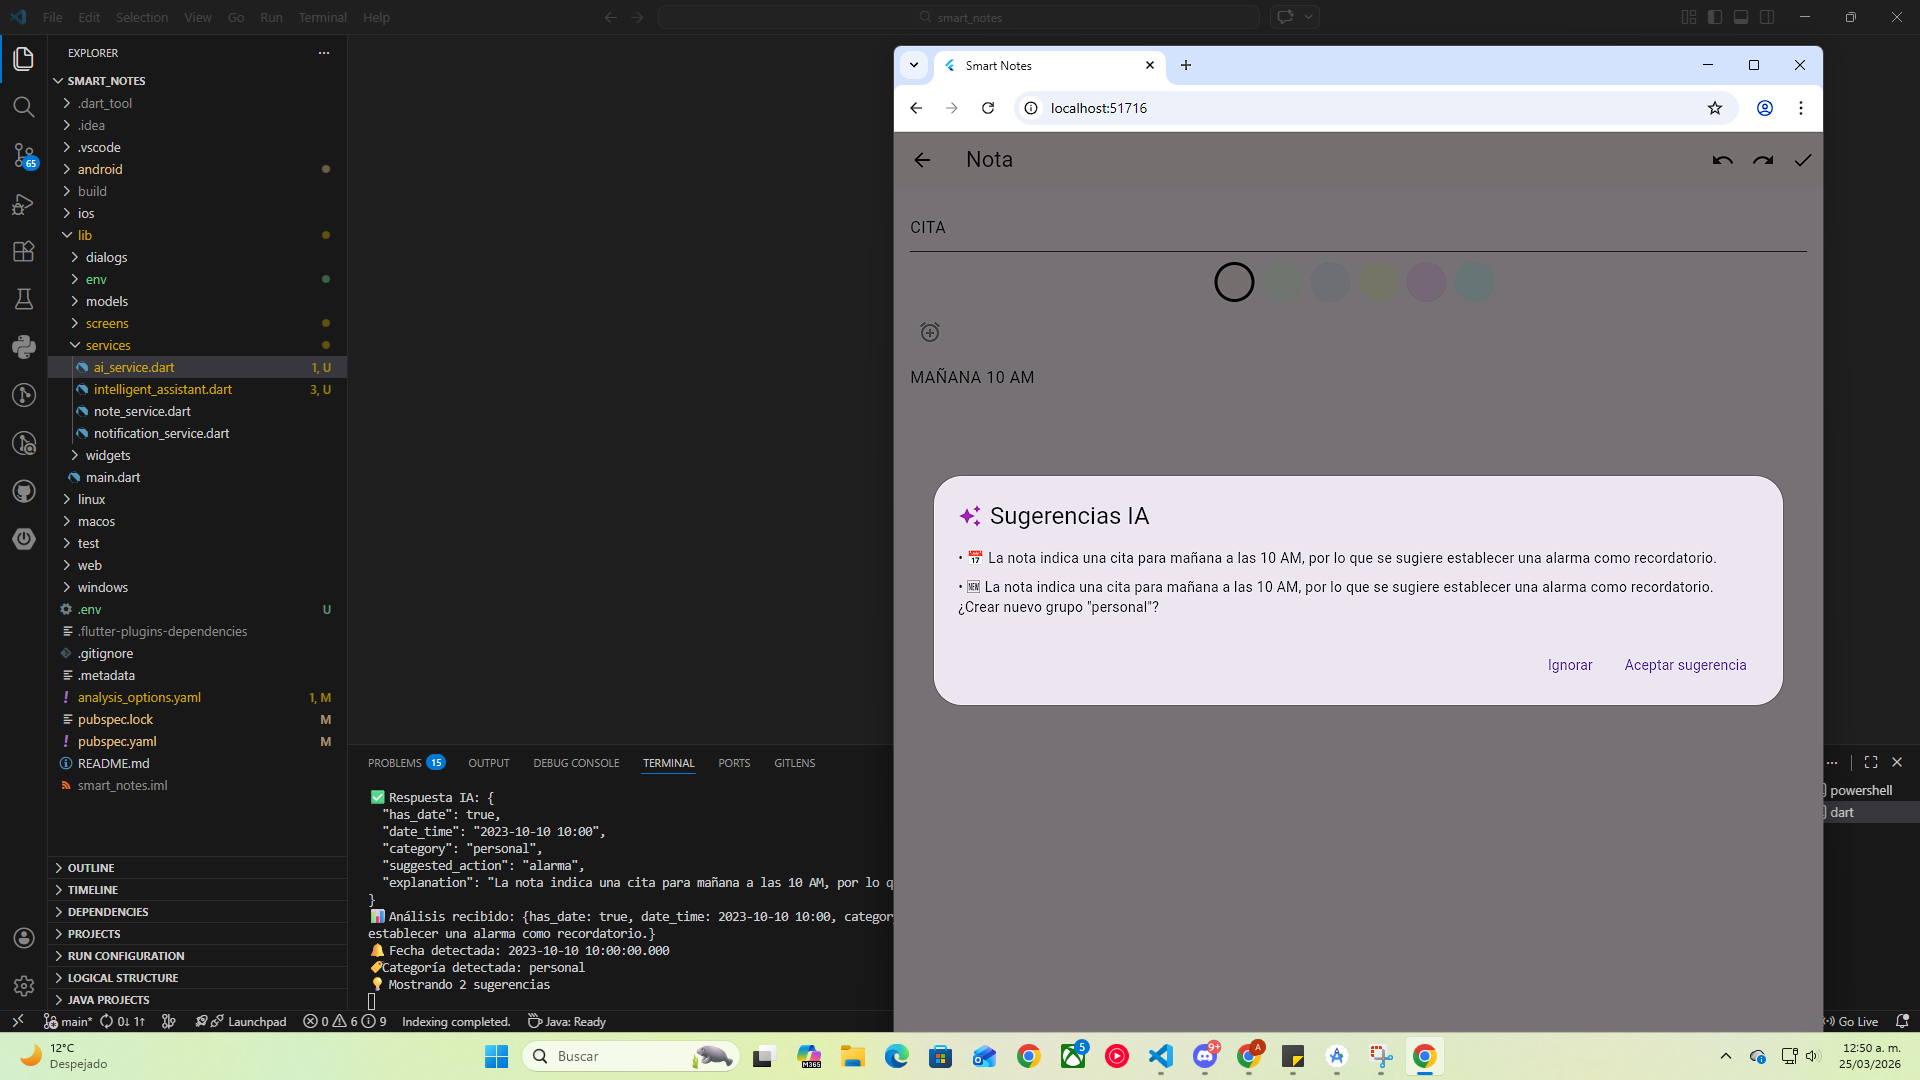
\includegraphics[width=0.7\textwidth]{prueba1.png}
\end{frame}

% 6. Pruebas Realizadas (Incluye arrastrar y agrupar)
\begin{frame}{Pruebas Realizadas con la IA}
    \begin{enumerate}
        \item \textbf{Reunión con el equipo} → Sugerencia de alarma
        \item \textbf{Proyecto Flutter final} → Sugerencia de crear grupo ``trabajo''
        \item \textbf{Cita con el dentista} → Sugerencia de recordatorio
        \item \textbf{Recordar comprar leche} → Sugerencia general
    \end{enumerate}
    
    \vspace{0.5em}
    \centering
    \small{Arrastrar y soltar también fue probado exitosamente}
    
    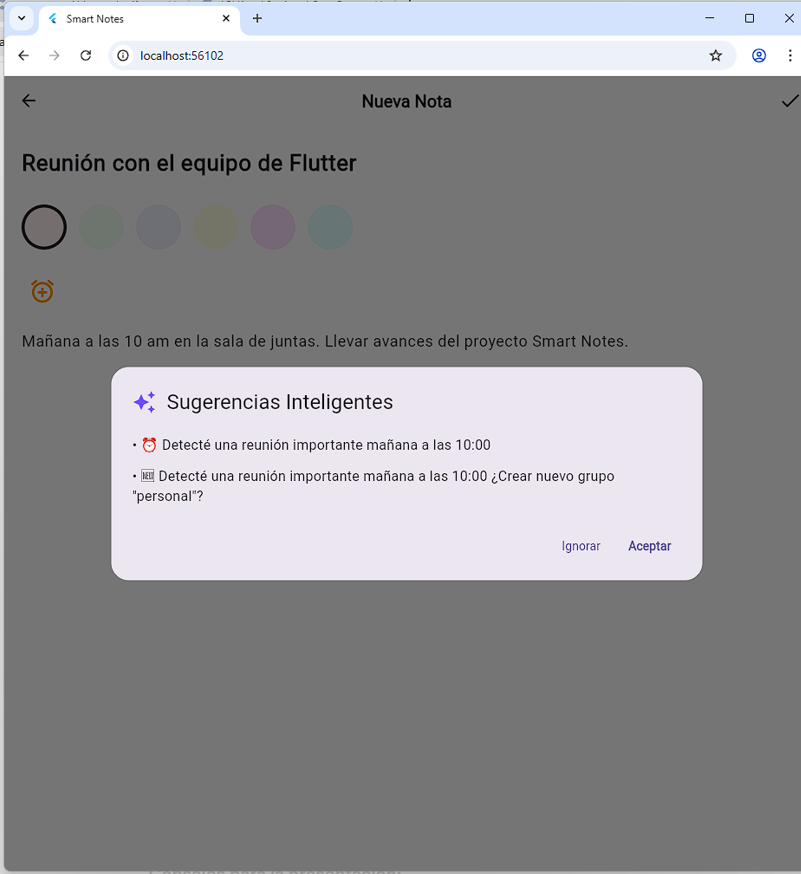
\includegraphics[width=0.45\textwidth]{prueba2.png}
    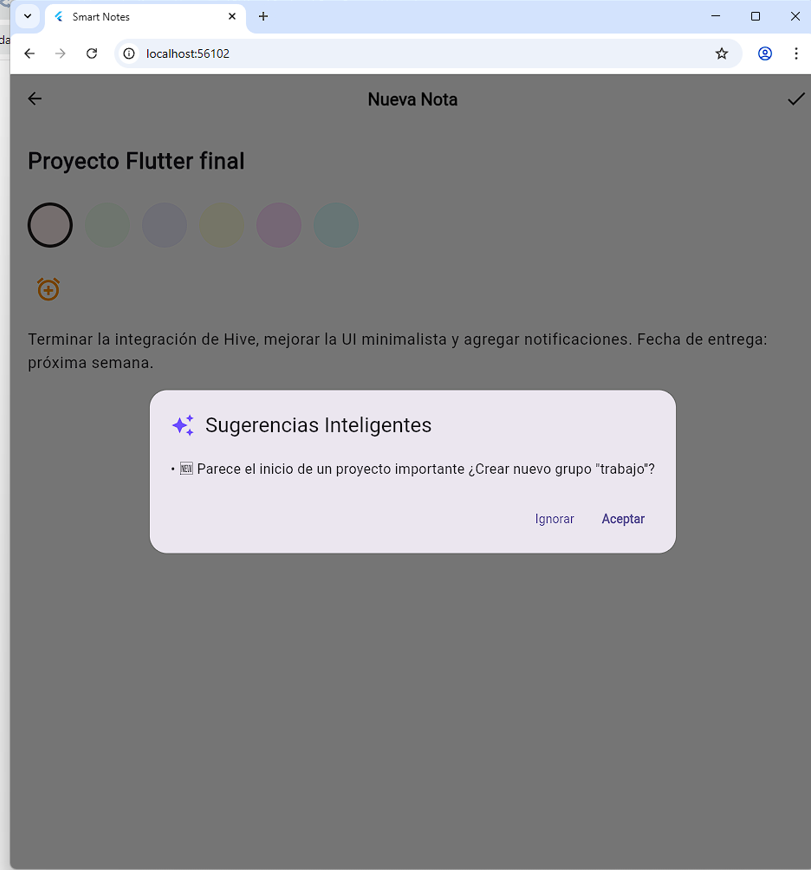
\includegraphics[width=0.45\textwidth]{prueba3.png}
\end{frame}

% 7. Configuración Manual
\begin{frame}{Configuración Manual de Alarmas}
    \begin{itemize}
        \item Además de las sugerencias de IA, se puede configurar manualmente
        \item Icono de alarma en la pantalla de edición
        \item Selector de fecha y hora nativo
        \item Notificaciones locales programadas
    \end{itemize}
    
    \centering
    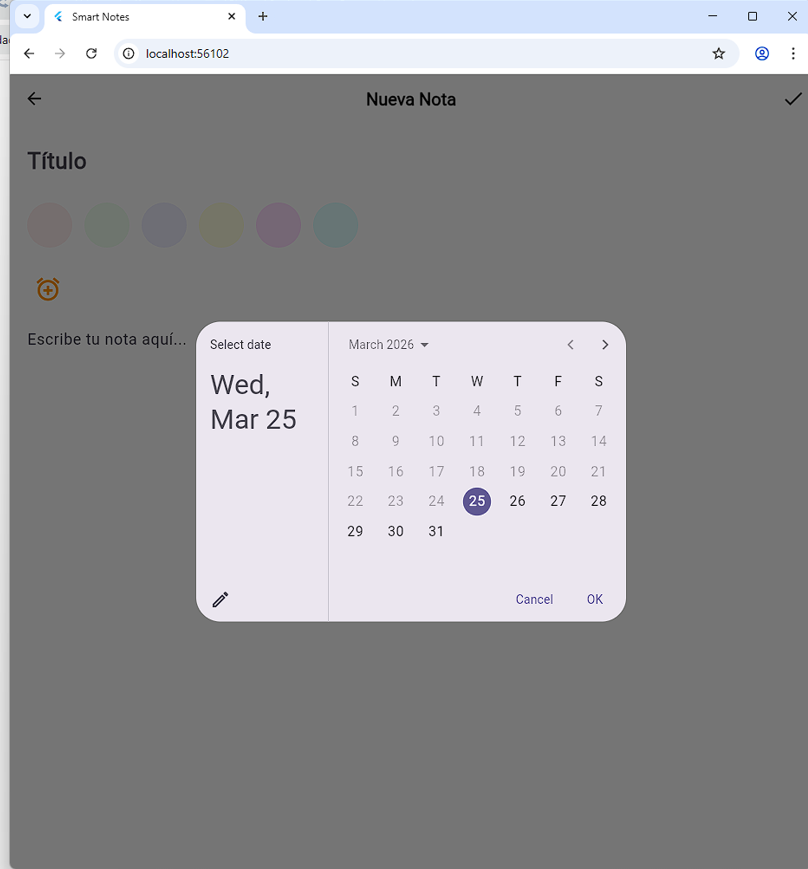
\includegraphics[width=0.65\textwidth]{configuracion_alarma.png}
\end{frame}

% 10. Conclusiones
\section{Conclusiones}
\begin{frame}{Conclusiones y Aprendizajes}
    \begin{itemize}
        \item Se logró una aplicación funcional, atractiva y con IA integrada
        \item La combinación de Flutter + Hive + OpenRouter resultó muy efectiva
        \item Se aplicaron correctamente principios de Interacción Humano-Computadora
        \item El arrastre y soltar + sugerencias inteligentes mejoran significativamente la experiencia de usuario
        \item Quedan áreas de mejora: OCR, voz, selección múltiple y sincronización en la nube
    \end{itemize}
    
    \vspace{1.5em}
    \centering
    {\Large \textbf{¡Gracias por su atención!}}
    
    \vspace{0.5em}
    Preguntas?
\end{frame}

\end{document}